\section{Shock-tubes}

In this section, we focus on simulation of soot formation in shock-tubes using the constant volume reactor of omnisoot, and compare species mole fraction and soot yield and morphology (if available) with benchmark measurements. Figure~\ref{fig:shocktubeschem} (left pane) illustrates the schematics of a shock-tube along with the idealized wave diagram. Shock-tubes are typically designed as a several meter long cylindrical tube separated by thin diaphragm into a smaller driver section filled a high pressure inert gas, and a longer driven section with diluted reactants. When the diaphragm is ruptured, the first shock wave propagates through the reactant mixture. The front shock compresses the reactants adiabatically raising the temperature and pressure throughout the shock-tube from $\mathrm{T_1}$, $\mathrm{P_1}$ to $\mathrm{T_2}$, $\mathrm{P_2}$. The passage of the reflected shock from the end wall heats up the reactants for the second time reaching $\mathrm{T_5}$, $\mathrm{P_5}$. Figure~\ref{fig:shocktubeschem} (right pane) shows the first and second jump in pressure due to the front and reflected shocks, respectively, and the variation in soot volume fraction during the pyrolysis of 0.03\% benzene in Ar. The reflected shock creates a nearly still mixture with a constant temperature and pressure (as shown in left pane of Figure~\ref{fig:shocktubeschem}) which provides an ideal condition for kinetic studies and rate constant investigations~\citep{kee2017chemically}. Therefore, the use of a shock tube provides a unique opportunity for investigating the kinetics of soot formation from fuels and at various temperatures, pressures and concentrations.

However, the processes investigated in shock tubes are limited to short residence times usually 1-3 ms, so they can only be used to study early stages of soot formation such as inception and surface growth, and not for processes occurring at longer residence times such as coagulation and carbonization. Note that the residence time is calculated after the passage of reflected shock. There is a delay in the increase of volume fraction known as induction time, $\mathrm{\tau_{ind}}$. There has been a lot of research in the literature focused on induction time (similarly on ignition delay time) in shock tubes~\citep{fussey1978shock}, but it is not the focus of this work. Instead, here we mainly investigate the species concentrations and soot characteristics during the pyrolysis of hydrocarbons, especially methane, at atmospheric and higher pressure which can be used for the design and optimization of carbon black in plasma reactors~\citep{fulcheri2023energy}. 

First, the pyrolysis of 5\% and 10\% $\mathrm{CH_4}$ diluted with Ar is investigated for the post-shock temperature range of 1800-3000 K and the pressure range of 4.7-7.1 bar. We assume the pressure linearly increase by temperature across the simulation cases. The obtained soot yields by were compared with the soot yield measured by \citet{agafonov2016unified} using a dual-beam absorption–emission technique. \citet{agafonov2016unified} reported yield$\times$E(m) at $\mathrm{\lambda}$=632~nm, and yield data was retrieved using E(m)=0.37 suggested therein. Figure~\ref{fig:shocktubeyield} depicts soot yield (SY) at the temperature dependence of  using Caltech~\citep{blanquart2009chemical}. Simulation were also performed using ABF~\citep{appel2000kinetic} and KAUST~\cite{wang2013pah} mechanisms, and the results were included in Appendix\hl{****}.

% run the shock-tube with other mechanisms and include the results in the Appendix

\begin{figure}[!htbp]
	\centering
	\begin{subfigure}[t]{0.4\textwidth}
		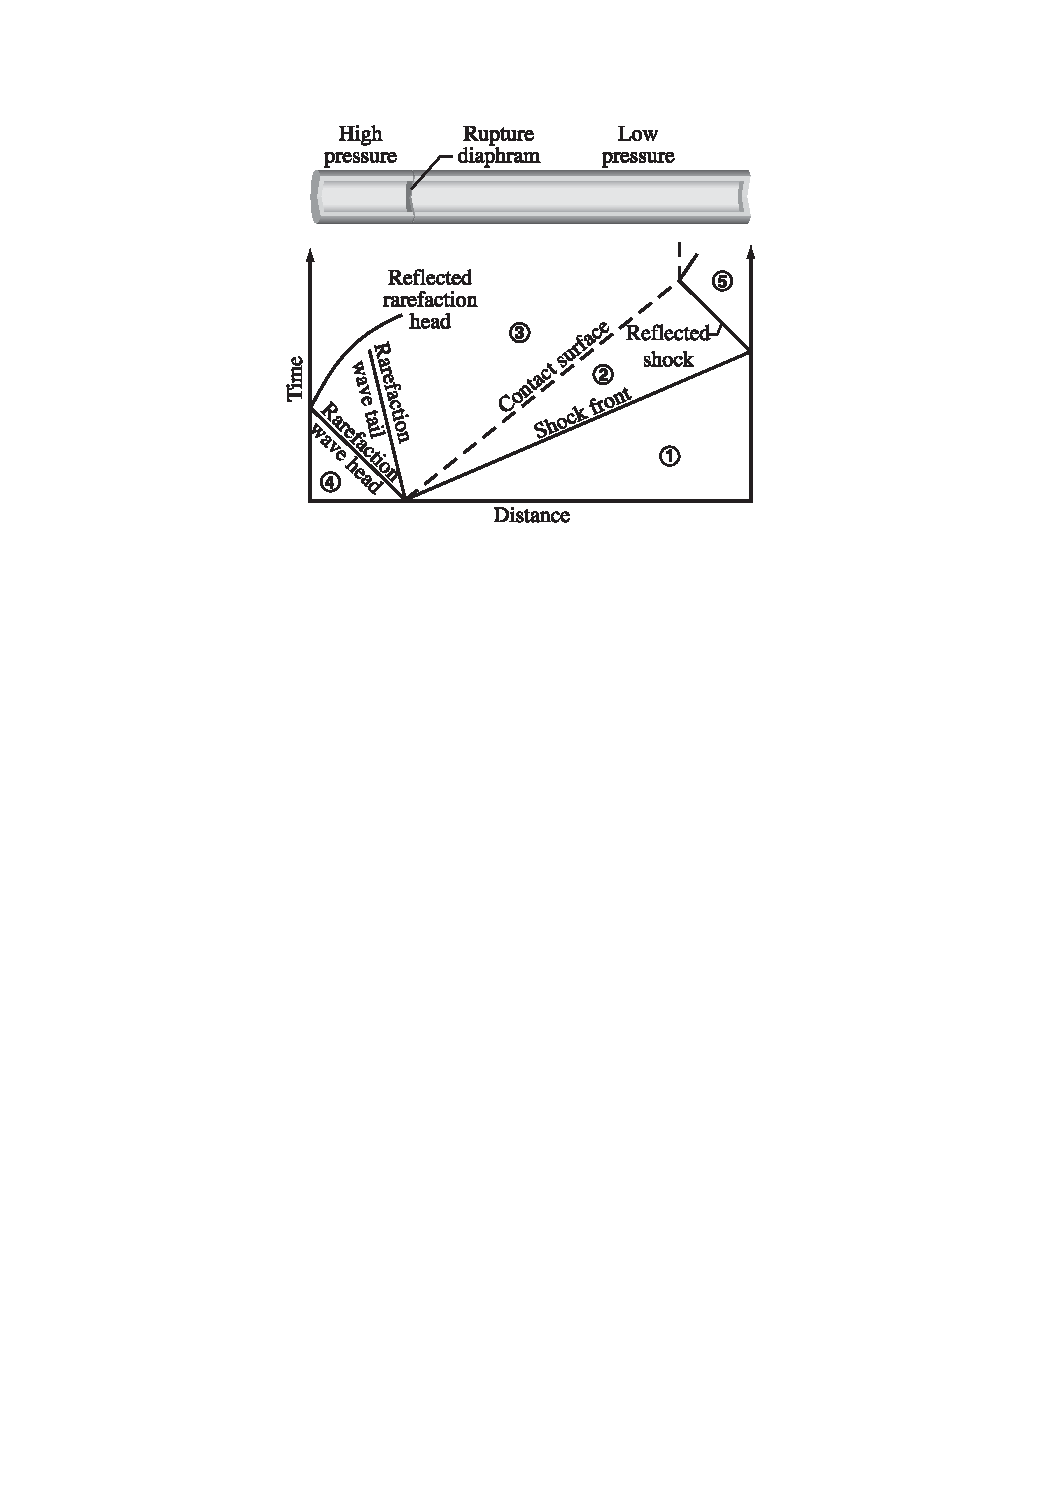
\includegraphics[width=1\textwidth]{Figures/Results/Shocktube/schematics.pdf}
	\end{subfigure}
	\begin{subfigure}[t]{0.4\textwidth}
	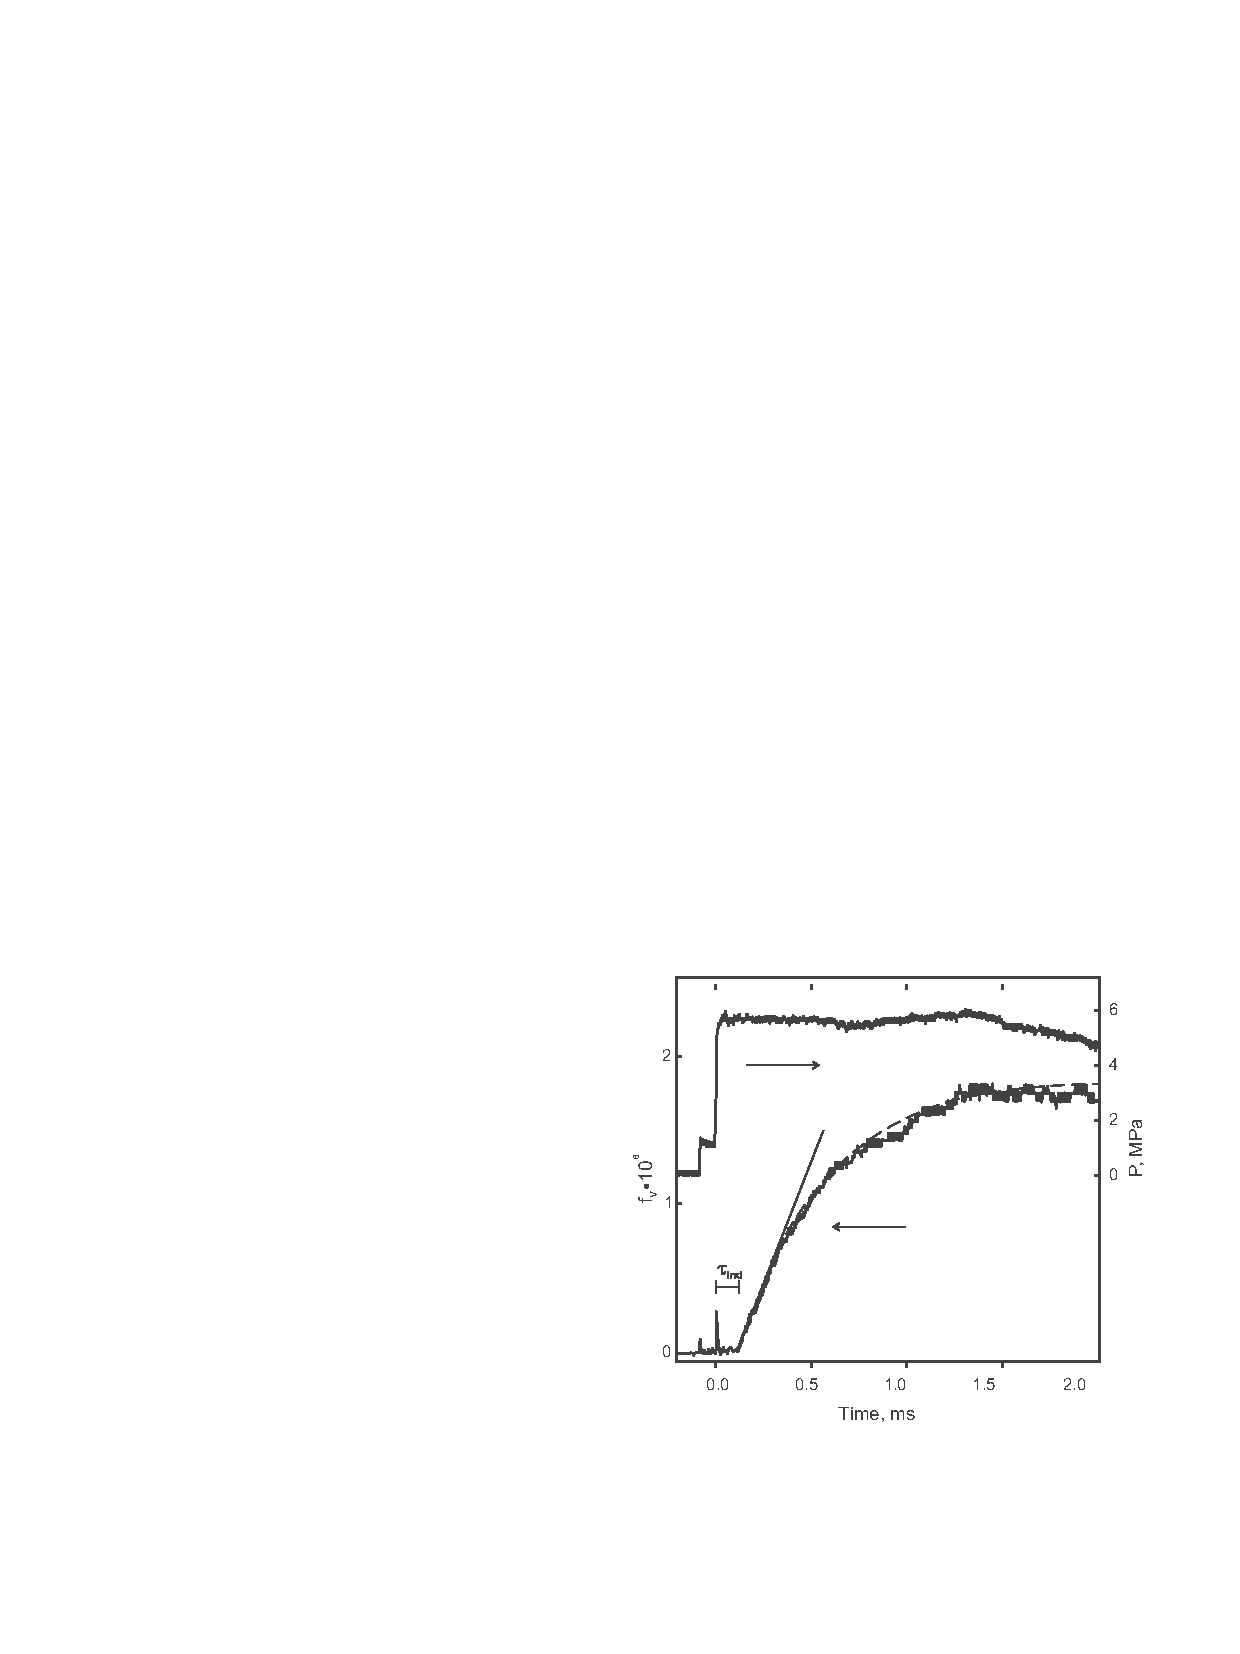
\includegraphics[width=1\textwidth]{Figures/Results/Shocktube/pfv_sample_shocktube.pdf}
	\end{subfigure}
	\caption{The schematics of a shock-tube and the idealized shockwave diagram(left pane reprinted from ~\citet{kee2017chemically}) and the variation of soot volume fraction measured by the extinction record at 633 nm and the pressure profile behind the reflected shock wave in a mixture 0.03\% benzene in Ar at T = 1890 K(right pane reprinted from ~\citet{karasevich1994soot})}
	\label{fig:shocktubeschem}
\end{figure}



\begin{figure}[H]
	\begin{subfigure}[t]{0.47\textwidth}
		\begin{tikzpicture}
			\draw (0, 0) node[inner sep=0] 	{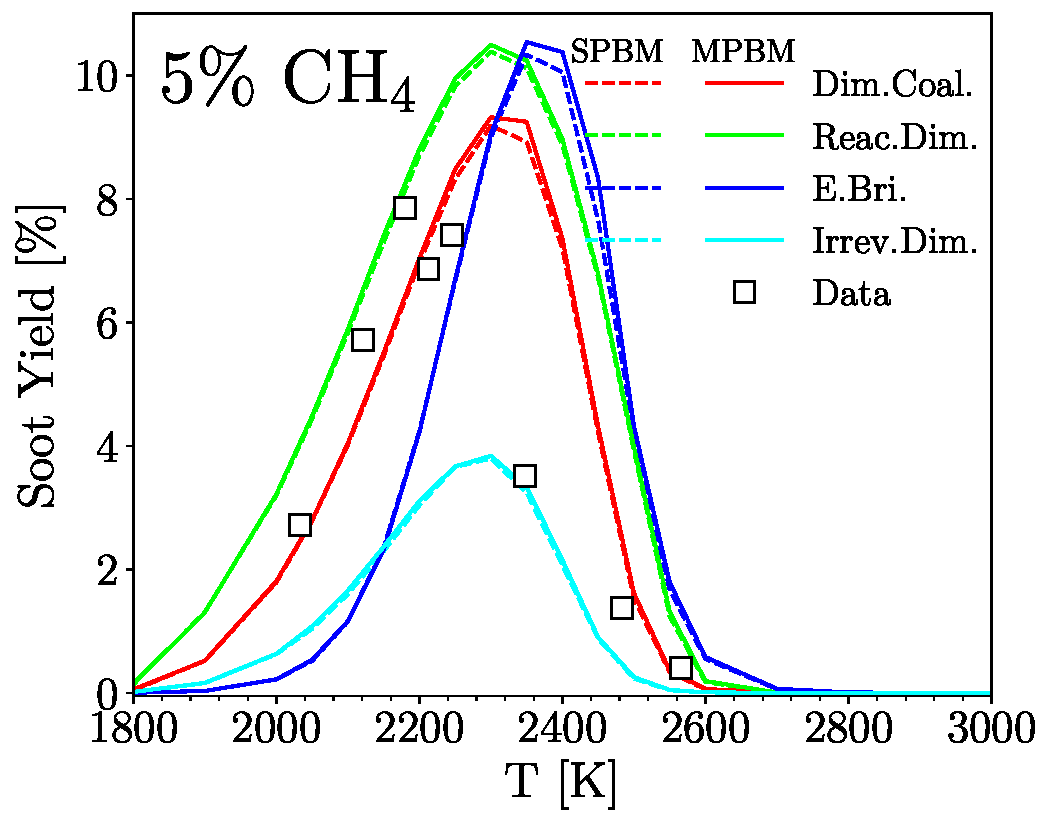
\includegraphics[width=1\textwidth]{Figures/Results/Shocktube/Agafonov2016/5CH4/carbon_yield.pdf}};
			\draw (2.65, 1.1) node {\scriptsize{\cite{agafonov2016unified}}};
		\end{tikzpicture}
	\end{subfigure}
	\begin{subfigure}[t]{0.47\textwidth}
	\begin{tikzpicture}
		\draw (0, 0) node[inner sep=0] 	{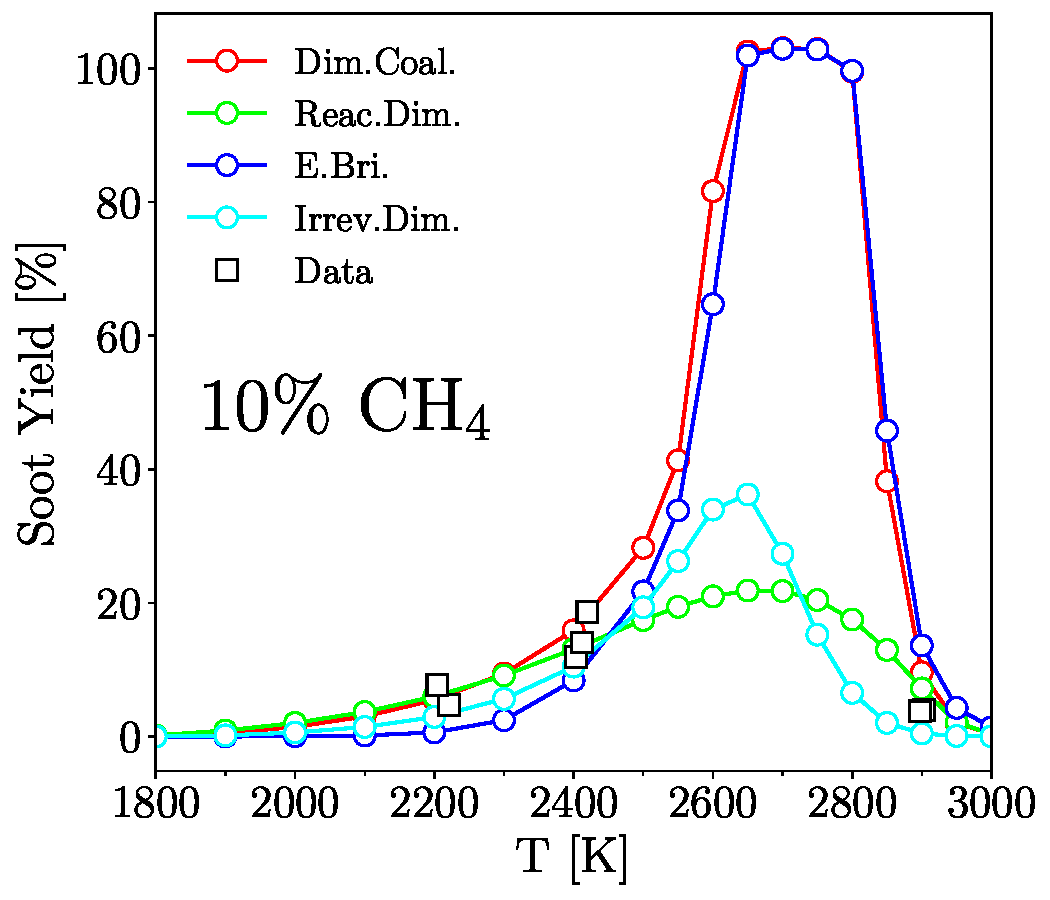
\includegraphics[width=1\textwidth]{Figures/Results/Shocktube/Agafonov2016/10CH4/carbon_yield.pdf}};
		\draw (-0.75, 1.2) node {\scriptsize{\cite{agafonov2016unified}}};
	\end{tikzpicture}
	\end{subfigure}
	\caption{The temperature dependence of soot yield during pyrolysis of 10\%~$\mathrm{CH_4}$-Ar (left pane) and 5\%~$\mathrm{CH_4}$-Ar (right pane) at $\mathrm{P}$ = 4.5–6.7 bar obtained using Caltech mechanism and different inception models compared with measurements at 1.5ms~\cite{agafonov2016unified} where the absorption funtion of E(m)=0.37 is used to estimate soot yield.}
	\label{fig:shocktubeyield} 
\end{figure} 